\documentclass[exa]{exercise_5.0}

\deadline{02.12.2024}

\begin{document}


\section{Thermische Ausdehnung}
Wenn es irgentwo so aussehen sollte, als ob der Rechenweg übersprungen wurde, liegt das daran, dass er in Python gemacht wurde. Der ganze Code steht auf den letzen Seiten.
\subsection{}
Der Gleichgewichtsabstand liegt bei $r_0 = 2^{\frac16}\sigma$. 
\begin{align*}
    V(r)&\peq V(r_0) + \frac{D_2}{2}(r-r_0)^2 + \frac{D_3}{3!}(r-r_0)^3 + \bigO{(r-r_0)^4}
\end{align*}
\begin{align*}
    \implies D_2 &= \pp[2]Vr\eval_{r_0} = \frac{72\epsilon}{r_0^2} = \frac{36\cdot 2^\frac23 \epsilon}{\sigma^2}\\
    \implies D_3 &= \pp[3]Vr\eval_{r_0} = -\frac{1512\epsilon}{r_0^3}= -\frac{756\sqrt 2\epsilon}{\sigma^3}
\end{align*}

\subsection{}
Die Ausweitung der Integrationsgrenzen auf $(-\inf,\inf)$ eigenet sich als Näherung, weil für $\abs{r-r_0}\gg1$ der Integrand exponentiell unterdrückt wird. 
\begin{align*}
    \tug x_T &= \frac{\int \dx x e^{-\beta U(x)}}{\int \dx e^{-\beta U(x)}}\\\\
    e^{-\beta U} &\approx e^{-\beta\hug{\frac{D_2}{2}(x-x_0)^2 + \frac{D_3}{3!}(x-x_0)^3}}
    \approx e^{-\beta\frac{D_2}{2}(x-x_0)^2}\hug{1-\beta \frac{D_3}{3!}(x-x_0)^3}\\
    \\
    \int_0^\inf \dx e^{-\beta U} &\approx \intR \dx e^{-\beta\frac{D_2}{2}(x-x_0)^2}\hug{1-\beta \frac{D_3}{3!}(x-x_0)^3}
    = \frac{2^{\frac16}\sqrt \pi \sigma}{6\sqrt{\beta\epsilon} }\\
    \\
    \int_0^\inf \dx xe^{-\beta U} &\approx \intR \dx x e^{-\beta\frac{D_2}{2}(x-x_0)^2}\hug{1-\beta \frac{D_3}{3!}(x-x_0)^3}
    = \frac{2^{\frac13}\sqrt \pi \sigma^2 ( 48\beta \epsilon + 7)}{288 \beta^\frac32 \epsilon^\frac32}\\
    \\
    \implies \Aboxed{\tug x_T &\approx 2^\frac16 \sigma\hug{1+ \frac{7}{48\beta \epsilon}}}
\end{align*}

\subsection{}
\begin{align*}
    l &= l_0 (1+\alpha \Delta T)= N\tug x_T\\
    &= N 2^\frac16 \sigma\hug{1+ \frac{7k_B T}{48\epsilon}}\\
    \implies \Aboxed{\alpha &= \frac{7k_B }{48 \epsilon} \approx 0.00126 \ufrac 1K}
\end{align*}
Der Ausdehnungskoeffizient hängt nicht von $\sigma$ ab, und befindet sich mit $\sim10^{-3} \ufrac 1K$ in der typischen Größenordnung für Flüssigkeiten. 

\section{Zweiatomige vs. einatomige lineare Kette}
\subsection{}
\begin{figure}[H]
    \centering
    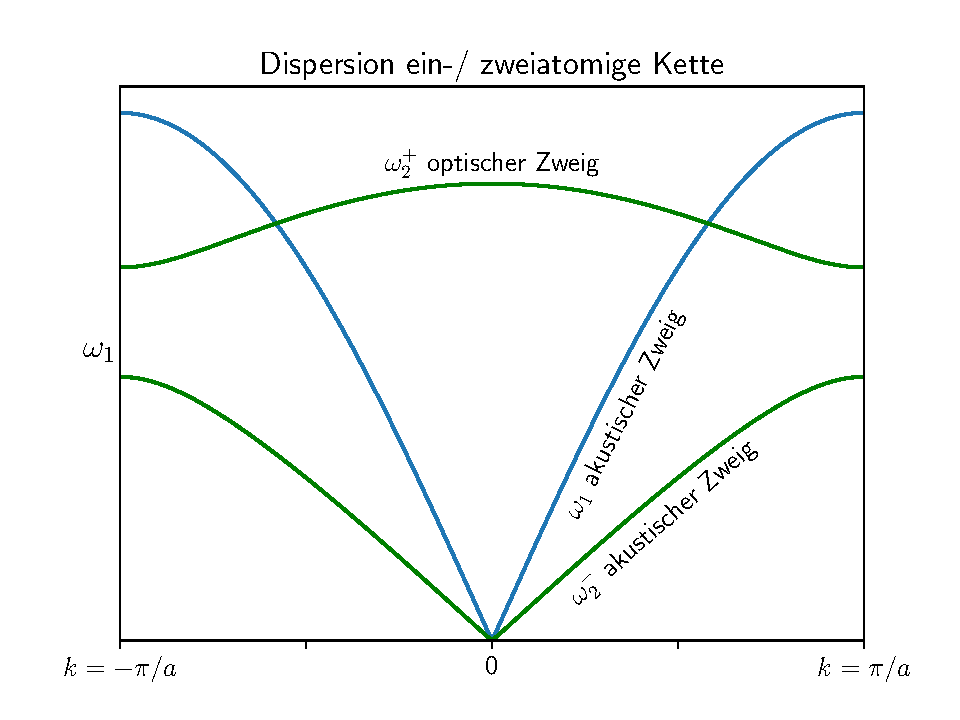
\includegraphics[width=0.8\textwidth]{dispersion.pdf}
    \caption{Dispersionskurve $\omega_2^\pm$ mit $M=2m$}
\end{figure}
Beide Dispersionskurven 
\begin{itemize}
    \item haben einen (qualitativ identischen) optischen Zweig 
    \item sind im $k$-Raum periodisch mit der Periode $\frac{2\pi}a$.
\end{itemize}
und unterschieden sich darin, dass 
\begin{itemize}
    \item die Dispersionkurve zu $\omega_2$ zu jedem $k$ eine zweite Lösung hat, welche auf dem optischen Zweig liegt
    \item es nur bei $\omega_2$ Bandlücken gibt (zwischen den beiden Zweigen).
\end{itemize}

\subsection{}
\begin{figure}[H]
    \centering
    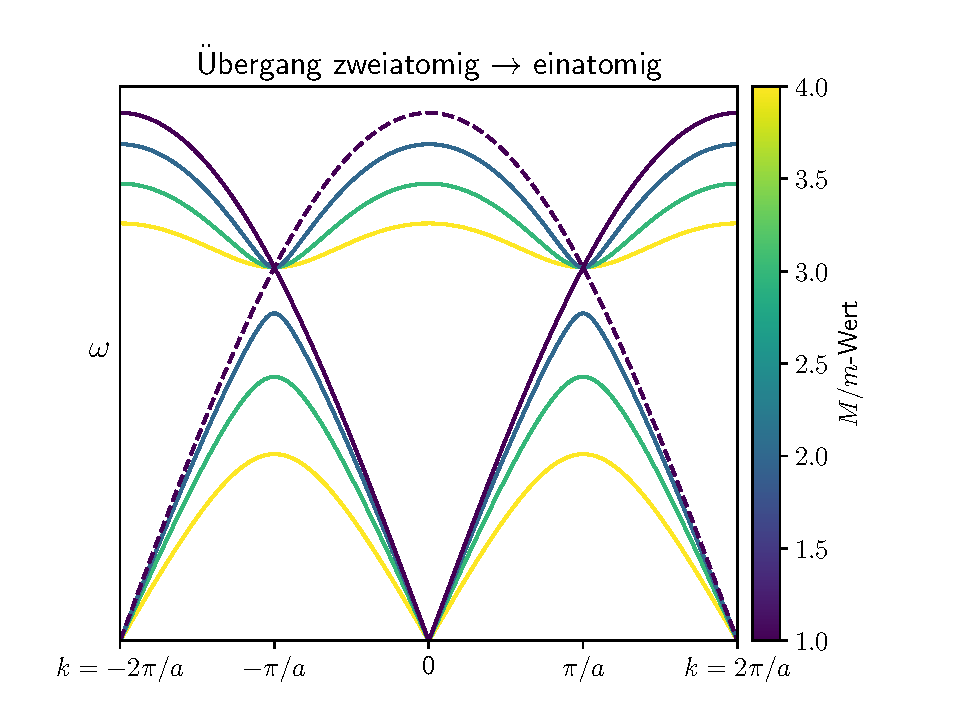
\includegraphics[width=.9\textwidth]{transition.pdf}
\end{figure}
Man kann im Plot sehen, wie sich die Dispersionkurve der zweiatomigen Kette, der der einatomigen annähert. Die Frequenzlücke wird immer kleiner, bis sie verschwindet. Im Fall dass $M=m$ ändert sich schlagartig die Größe der Einheitszelle $a\to a/2$, sodass man hier die Achsen neu definieren muss.

\section{Kette mit verschiedenen Federn}
\subsection{}
\begin{align*}
    \omega_- &=\sqrt{ \frac{D_1+D_2}{m} - \frac1{m}\sqrt{D_1^2 + D_2^2 + 2D_1D_2 \cos(ka)}}\\
   v &= \limn k\pp{\omega_-}k \\
   &= \limn k\frac{D_1D_2 a \sin(ak)}{2m \sqrt{\frac{D_1 +D_2}{m} - \frac1m \sqrt{D_1^2 + D_2 ^2 + 2 D_1 D_2 \cos(ak)}} \sqrt{D_1^2 + D_2^2 + 2D_1 D_2 \cos(ak)}}  \\  
   &= \limn k\frac{D_1D_2 a^2 k}{2\sqrt m \sqrt{D_1 +D_2 - \hug{D_1 + D_2 - \frac{D_1 D_2 a^2 k^2}{2(D_1 + D_2)}} } (D_1 + D_2)}  \\  
   &= \frac{D_1D_2 a}{\sqrt {2m}\sqrt{\frac{D_1 D_2}{(D_1 + D_2)} } (D_1 + D_2)}  \\  
   \Aboxed{v&= \sqrt{\frac{a^2 D_1D_2 }{2m(D_1 + D_2)}}}  
\end{align*}

\subsection{}
Der Term ist 2 mal das harmonisches Mittel der Federkonstanten und stellt eine effektive Federkonstante dar, die die Wechselwirkung zwischen den beiden benachbarten Atomen in der Kette beschreibt. 

\section{Phononen in Cu}
\subsection{}
\begin{align*}
    v &= a\sqrt{\frac{D}{m}},\qquad 
    \omega\sub{max} = \omega(k=\pi/a) 
    = 2\sqrt{\frac Dm} = \frac {2v}a
\end{align*}
\begin{align*}
    \Aboxed{\omega\sub{max}&\approx 23.8\u{THz}}
\end{align*}

\subsection{}
\begin{align*}
    \Aboxed{E\sub{max} = \hbar\omega\sub{max} \approx 15.7\u{meV}} 
\end{align*}

\section{Streuung von Licht an Schallwellen (Brillouin-Streuung)}
\subsection{}
\begin{align*}
    k\sub{photon} &= n k_0 
    = n \frac{2\pi}{\lambda}
    \approx 13.9\E{6} \frac1m\\
    \Delta k\sub{max} &= 2 k\sub{ph} \approx 27.9\E6\ufrac1m\\
    \Aboxed{\Delta p\sub{max} &= \hbar\Delta k \sub{max} \approx 2.94\E{-27}\ufrac{kg\, m}{s}}
\end{align*}

\subsection{}
\begin{align*}
\Aboxed{\omega\sub{phonon} = v \Delta k\sub{max} \approx 167\u{GHz}}
\end{align*}

\subsection{}
\begin{align*}
    \Aboxed{\frac{\Delta E}{E} &= \frac{\omega\sub{phonon}}{\omega\sub{photon}} \approx 6.16\E{-5}}
\end{align*}

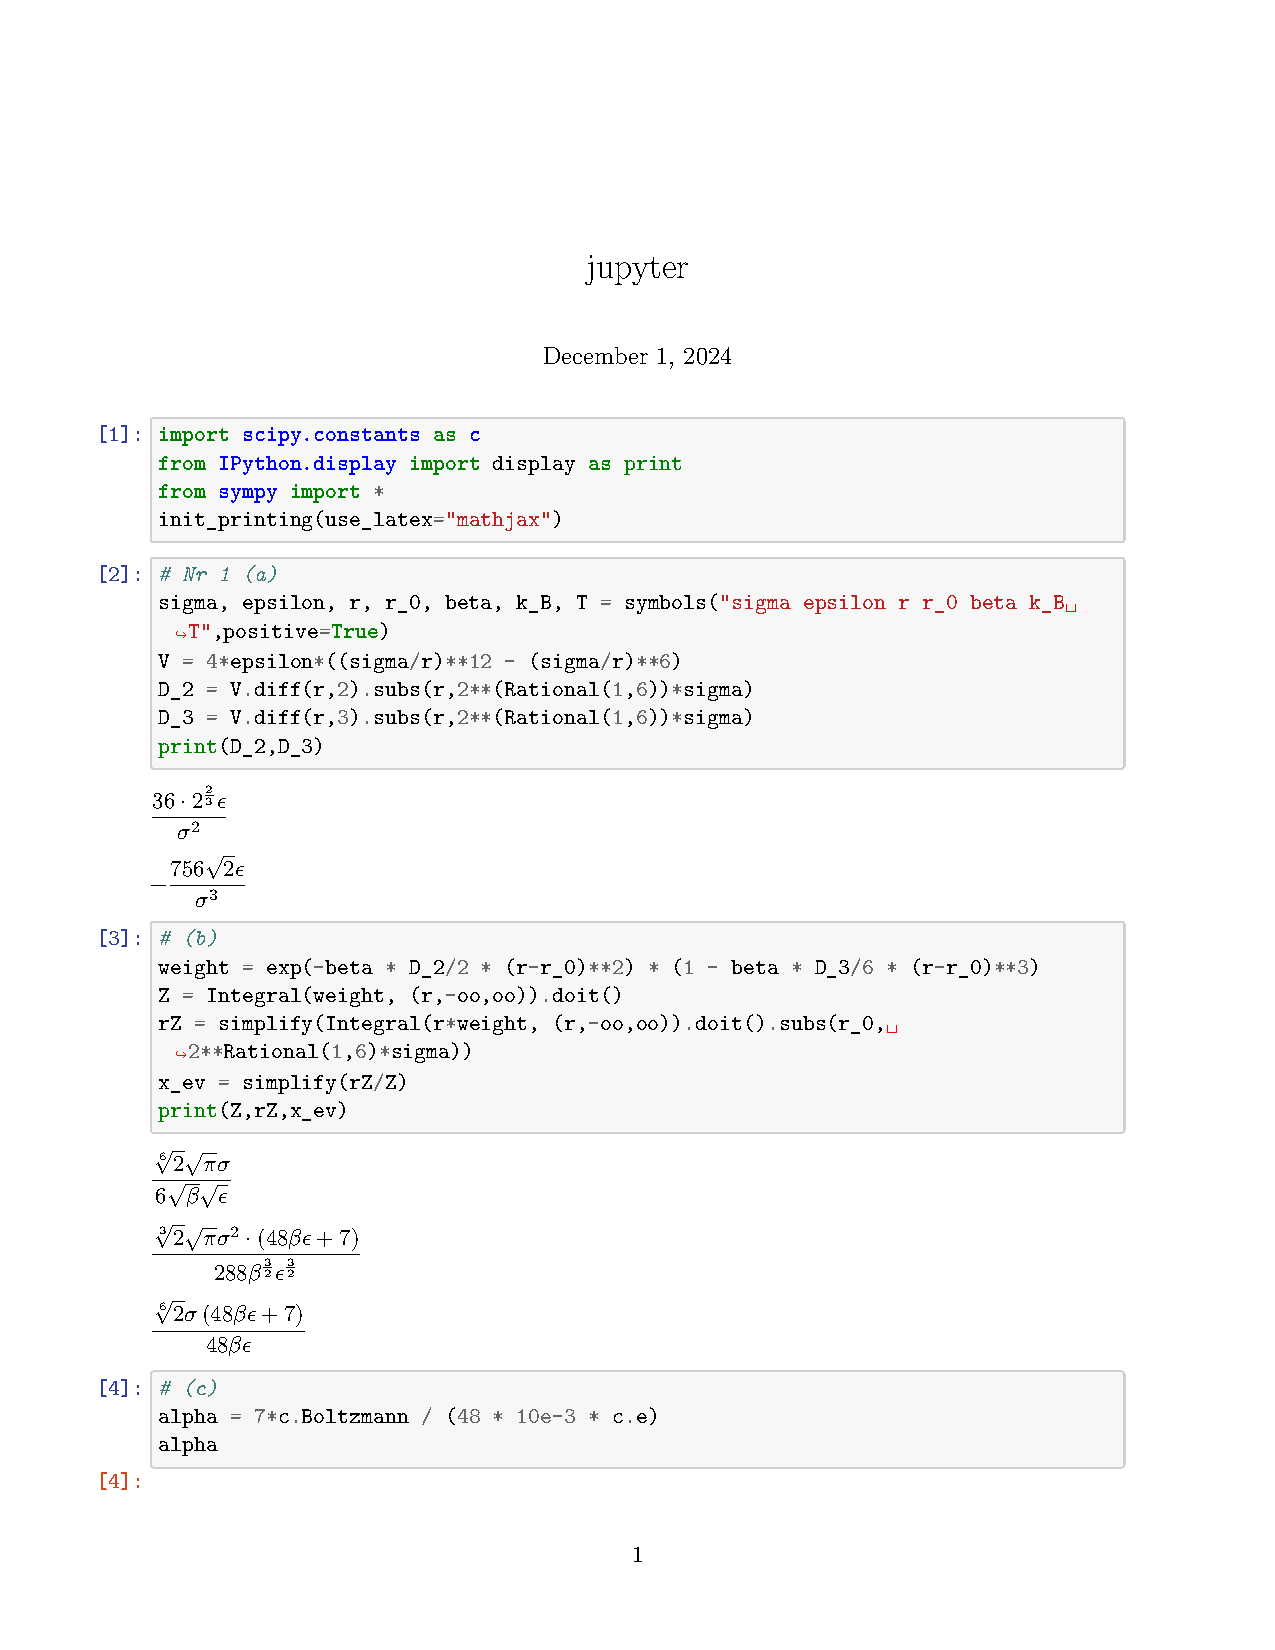
\includepdf[pages=-,link=true, linkname=py]{jupyter.pdf}

\end{document}